\chapter{Supersymmetry \label{chap:supersymmetry}}

Supersymmetry is a space-time symmetry that relates fermions and bosons. The operator $Q$
generating the transformation from fermion to boson and vice versa is an anti-commuting spinor, with
\begin{align}
  Q \Ket{\textrm{Boson}} &= \Ket{\textrm{Fermion}} \\
  Q \Ket{\textrm{Fermion}} &= \Ket{\textrm{Boson}} .
\end{align}
From the above we can immediately see that $Q$ must be fermionic in nature, and carries spin 1/2. 
The generator $Q$ and its hermitian conjugate $Q^\dagger$ satisfy the anticommutation and
commutation relations
\begin{align}
  \{Q,Q^\dagger\} &= P^\mu ,\\
  \{Q,Q\} &= \{Q^\dagger,Q^\dagger\} = 0, \\
  \left[P^\mu,Q\right] &= \left[P^\mu,Q^\dagger\right] = 0 ,
\end{align}
with $P^\mu$ the four-momentum generator of spacetime translations. 
Particles in a supersymmetric theory fall in the irreducible representations of the SUSY algebra,
the supermultiplets, which contain both a fermion and a boson. 
Since the SUSY generators commute with $P^2$, it follows that the particles within a given
supermultiplet have the same mass. Since we have not experimentally observed any of these new
particles, this implies that SUSY must be a broken symmetry. 
Given that $Q$ and $Q^\dagger$ also commute with the generators of the gauge transformations, 
particles in the same supermultiplet must have the same gauge quantum numbers. 

Supersymmetry was originally introduced~\cite{Wess,Golfand,Chamseddine,Kane,Fayet,Barbieri,Hall} to
help construct a grand unified theory (GUT), merging all known forces in a single framework. For
this to occur, there needed to be a link between particles of different spin. In this context it is
also noteworthy to mention that the coupling constants appear to unify at around
$\text{10}^\text{16}\GeV$ if we include contributions from supersymmetry in the renormalization
group equations. Making SUSY a local symmetry results into supergravity, which is the first step to
including gravity in the overall unified framework. 

Nowadays, supersymmetry receives much attention due to the solution it can provide for the
hierarchy problem, and the dark matter candidate that is present in many SUSY models. If SUSY is to
be the solution to the hierarchy problem, then this also means that at least some of the
supersymmetric partners (superpartners) of the ordinary SM particles should be produced at the LHC
energies. This is what motivates the many SUSY searches performed at the CMS and ATLAS experiments,
including the search presented in this thesis. 

In this chapter I will first provide some general considerations on possible supermultiplets and
SUSY breaking mechanisms in Sections~\ref{sec:susy_supermultiplets} and \ref{sec:susy_breaking}. 
Then, I will focus on the so-called Minimal Supersymmetric Standard Model (MSSM) in
Section~\ref{sec:susy_MSSM}, covering its particle content, and introducing the concept of
R-parity. Section~\ref{sec:susy_EWbreaking} will explain how to break the electroweak symmetry in
a supersymmetry context. The production and decay of superpartners along with their basic
experimental signatures are presented in Section~\ref{sec:susy_sparticles}. 
The last two sections cover topics that are of particular importance to the razor boost analysis. 
Section~\ref{sec:susy_natural_susy} will cover natural SUSY and how it will solve the hierarchy
problem. The concluding section in this chapter will cover the simplified approach that is
used by experiments to guide new physics searches and present results. 
The bulk of this chapter is based on the excellent review by S. Martin~\cite{Martin:1997ns}. 

\section{Supermultiplets \label{sec:susy_supermultiplets}}

Particles in a supersymmetric theory are represented by the supermultiplets, also called
superfields. These are spin multiplets which contain both fermion and boson states. From the
spin-statistics theorem it follows that there must be an equal number of fermionic and bosonic
degrees of freedom. 
Interactions between particles can be most elegantly formulated in terms of the superfields, rather
than the separate components. Superfields live in superspace, an extension of the
usual spacetime with fermionic (Grassmann) variables. A detailed discussion of the superfield
formalism is, however, beyond the scope of this thesis. Interested readers are referred to
Refs.~\cite{Martin:1997ns,Polonsky:2001pn}. 

The simplest possibility for a supermultiplet consists of a two-component Weyl fermion and a complex
scalar field, the sfermion. It is called a \textit{chiral} or \textit{matter supermultiplet}. The
ordinary SM fermions fit into these chiral multiplets, albeit that the left- and right-handed
fermions need to reside in different multiplets. 

A second possibility is to include a spin-1 vector boson. The resulting supermultiplet is
called a \textit{gauge} or \textit{vector supermultiplet} and consists of a massless spin-1 boson
and a massless spin-1/2 Weyl fermion. The bosons can only attain a mass through spontaneous
symmetry breaking if the theory is to remain renormalizable. 
Given that gauge bosons transform under the adjoint representation of the gauge
group, so must their superpartners, the so-called gauginos. This means that left-handed and
right-handed gauginos will transform the same under the gauge group as opposed to the fermions we
know from the Standard Model. 

There are other possibilities to construct supermultiplets, but if they have renormalizable
interactions they can all be reduced to chiral and gauge supermultiplets. Hence, these will not be
considered here. 
How all SM particles fit inside the supermultiplets will be discussed in
Section~\ref{sec:susy_MSSM_particles}, when introducing the particle content of the MSSM. 


\section{Supersymmetry breaking mechanisms \label{sec:susy_breaking}}

Unbroken supersymmetry leads to superpartners with the same mass as the normal SM particles, and
which would thus have been discovered a long time ago. Since this is not the case,
supersymmetry, assuming it exists, must be broken such that the superpartners have a large mass
and would have avoided detection. 

As we will see shortly, this has an influence on the discussion of the hierarchy problem in a SUSY
context. 
When assuming perfect supersymmetry, there is no correction to the Higgs boson mass at all. When
supersymmetry is broken, on the other hand, this cancellation no longer happens.
In order to avoid the reappearance of quadratic divergencies, we can only allow \textit{soft SUSY
breaking}. 
This means that the relations between the dimensionless coupling constants (e.g. $\lambda_S =
|\lambda_f|^2$, cf. Section~\ref{sec:hierarchy_problem}) must still hold. 
If this is the case we will only have logarithmically divergent terms contributing to the Higgs mass
correction, which will be of the form
\begin{equation}
  \Delta m_H^2 = m_{\text{soft}}^2 \left(\frac{\lambda}{16 \pi^2}
\ln{\frac{\Lambda}{m_{\text{soft}}} + \ldots}\right) ,
\end{equation}
with $m_{\text{soft}}$ the mass scale associated with the soft terms, $\lambda$ a schematic
representation of various couplings and where the ellipses include higher order loop corrections and
terms independent of the ultraviolet cutoff scale $\Lambda$. 
Therefore, the masses of the superpartners cannot be too huge, otherwise the $m_{\text{soft}}^2$
corrections to the Higgs mass would become unnaturally large again. 
%One finds that the masses of at least the lightest superpartners should be at most of the order of
%$1~\textrm{TeV}$.

Unfortunately, breaking SUSY softly is not so easy, and, up to now, nobody has found a
satisfactory way to do it dynamically. There are several ideas, which are mostly based on the idea
that SUSY is broken in a different sector, and then communicated to the visible sector by some form
of mediator particles. The two main classes of mediator mechanisms are via gravitational
interactions, or via the gauge interactions. 

Because of these difficulties, the possible soft SUSY breaking terms are usually added to the
Lagrangian by hand, 
\begin{equation}
  \mathcal{L} = \mathcal{L}_{\text{SUSY}} + \mathcal{L}_{\text{soft}},
  \label{eq:L_general}
\end{equation}
resulting in a low-energy effective theory. This effective theory can then be
used to predict masses, decays etcetera. The downside is of course that the parameters governing
the soft breaking terms are mostly unconstrained. 

%%%%%%%%%%%%%%%%%%%%%%%%%%%%%%%%%%%%%%%%%%%%%%%%%%%%%%%%%%%%%%%%%%%%%%%%%%%%%%%%%%%%%%%%%%%%%%%%%%

\section{Minimal Supersymmetric Standard Model \label{sec:susy_MSSM}}

\subsection{Particle content \label{sec:susy_MSSM_particles}}

A first step to building a minimal supersymmetric extension of the Standard Model, is to fit all the
SM particles in supermultiplets. 
Standard Model fermions -- the quarks and leptons -- have to be members of chiral supermultiplets,
because left- and right-handed fermions transform differently under the electroweak gauge symmetry.
Their spin-0 superpartners are called squarks and sleptons, where `s' stands for scalar.
Symbolically, superpartners are denoted with a tilde above the usual SM symbol. 
Often a `handedness' is also assigned to the superpartners, but it is important to remember that
they are scalars, and so the concept of helicity is ill-defined. The handedness in this case is
just a label referring to their SM partners. 

The Higgs fields are spin-0 fields, and so they will also reside in a chiral supermultiplet. The
fermionic partner of the Higgs field is called a higgsino. As it turns out, one Higgs chiral
supermultiplet is not enough in supersymmetry. Two such multiplets are needed for two main reasons. 
\begin{enumerate}
  \item Anomaly cancellation: an anomaly occurs when a classical symmetry of the Lagrangian is not
conserved at the quantum level. If this happens for a gauge symmetry, this causes the theory to be
inconsistent. The specific particle content of the SM results in an anomaly free gauge symmetry
because the condition $\text{Tr}[T^2_3 Y] = \text{Tr}[Y^3] = 0$, with the trace running over the
left-handed Weyl fermionic degrees of freedom in the theory, is satisfied. 
A higgsino must have either hypercharge $Y = +1/2$, or $Y=-1/2$. By itself, the introduction of a
higgsino would thus spoil the nice cancellation in the trace. To restore it, we need two Higgs
supermultiplets with opposite hypercharge. 

  \item Structure of supersymmetric theories: only a $Y = +1/2$ Higgs chiral supermultiplet can have
the Yukawa couplings needed to give masses to up-type quarks and, similarly, only a $Y = -1/2$ Higgs
can give mass to down-type quarks and charged leptons.
In the SM, the conjugate of the Higgs field is used to give mass to the down-type quarks, but this
is no longer possible in SUSY because the conjugate would have the wrong chirality.
\end{enumerate}
The two Higgs supermultiplets will be denoted by $H_u$ and $H_d$, for $Y = +1/2$ and $Y = -1/2$,
respectively.  

The chiral supermultiplets present in the MSSM are summarized in Table~\ref{tab:chiral_multiplets}.
The representation of the Standard Model gauge group under which the supermultiplets transform is
given in the last column.
All chiral supermultiplets are defined in terms of left-handed Weyl spinors, which is why the
conjugates of the right-handed quarks and leptons appear in the table.

\begin{table}[t]
  \caption{Chiral supermultiplets in the MSSM with their gauge quantum numbers.}
  \begin{center}
  \begin{tabular}{ l c | c c c }
    \toprule
    \multicolumn{2}{l}{Names} & Spin 0 & Spin 1/2 & $SU(3)_c \times SU(2)_L \times U(1)_Y$ \\ 
    \midrule
    \multirow{3}{2cm}{squarks, quarks \\(3 families)} & $\widehat{Q}$ & ($\widetilde{\cPqu}_L \
\widetilde{\cPqd}_L$) & ($\cPqu_L \ \cPqd_L$) & ($\mathbf{3}, \mathbf{2}, \frac{1}{6}$)  \\[1ex] 
    & $\widehat{U}^c$ & $\widetilde{\cPqu}_R^*$ & $\cPqu_R^\dagger$ & ($\mathbf{\overline{3}},
\mathbf{1}, -\frac{2}{3}$)  \\[1ex]
    & $\widehat{D}^c$ & $\widetilde{\cPqd}_R^*$ & $\cPqd_R^\dagger$ & ($\mathbf{\overline{3}},
\mathbf{1}, \frac{1}{3}$)  \\ 
    \midrule
    \multirow{2}{2cm}{sleptons, leptons \\(3 families)} & $\widehat{L}$ & ($\widetilde{\nu} \
\widetilde{e}_L$) & ($\nu \ e_L$) & ($\mathbf{1}, \mathbf{2}, -\frac{1}{2}$) \\[1ex] 
    & $\widehat{E}^c$ & $\widetilde{e}_R^*$ & $e_R^\dagger$ & ($\mathbf{1}, \mathbf{1}, 1$) 
\\[1.2ex] 
    \midrule
    \multirow{2}{2cm}{Higgs, higgsinos} & $\widehat{H}_u$ & ($H_u^+ \ H_u^0)$ &
($\widetilde{H}_u^+ \ \widetilde{H}_u^0$) & ($\mathbf{1}, \mathbf{2}, +\frac{1}{2}$) \\[1ex] 
    & $\widehat{H}_d$ & ($H_d^0 \ H_d^-$) & ($\widetilde{H}_d^0 \ \widetilde{H}_d^-$)  &
($\mathbf{1}, \mathbf{2}, -\frac{1}{2}$) \\
  \bottomrule
  \end{tabular}
  \end{center}
  \label{tab:chiral_multiplets}
\end{table}

The vector bosons of the Standard Model will have to reside in gauge supermultiplets together with
a Majorana fermion field. An overview of the gauge superfields present in the MSSM is given in
Table~\ref{tab:gauge_multiplets}. 
% TODO: perhaps remove the next sentence (move to further section)
After electroweak symmetry breaking, the neutral gauge bosons
$\W^3$ and $B^0$ mix to form the mass eigenstates $\cPZ$ and $\gamma$. The corresponding gaugino
mixed states are called the zino ($\widetilde{\cPZ}$) and photino ($\widetilde{\gamma}$). 

\begin{table}[t]
  \caption{Gauge supermultiplets in the MSSM with gauge quantum numbers. }
  \begin{center}
  \begin{tabular}{ l c | c c c }
    \toprule
    \multicolumn{2}{l}{Names} & Spin 0 & Spin 1/2 & $SU(3)_c \times SU(2)_L \times U(1)_Y$ \\ 
    \midrule
    gluino, gluon & $\widehat{G}_a$ & $\widetilde{g}_a$ & $g^\mu$ & ($\mathbf{8}, \mathbf{1}, 0$)
\\[1ex]
    winos, $\W$ bosons & $\widehat{\W}_a$ & $\widetilde{\W}_a$ & $\W_a^\mu$ &
($\mathbf{1}, \mathbf{3}, 0$)  \\[1ex]
    bino, $B^0$ boson & $\widehat{B}$ & $\widetilde{B}$ & $B^\mu$ & ($\mathbf{1}, \mathbf{1}, 0$) \\
    \bottomrule
  \end{tabular}
  \end{center}
  \label{tab:gauge_multiplets}
\end{table}

It is interesting to observe that mass terms for the sfermions, higgsinos and gauginos are not
strictly forbidden. Squarks and sleptons are scalar fields, and a mass term $m^2|\phi|^2$ is always
allowed by gauge symmetries. For the higgsinos and gauginos this is allowed because they are
fermions in a real representation of the gauge group. 
The known SM particles on the other hand, would all be massless if not for the electroweak symmetry
breaking. Therefore, from the point of view of the MSSM, it does not come as a surprise that those
are the only particles that were light enough to be detected so far.  

\subsection{Supersymmetric Lagrangian \label{sec:susy_lagrangian}}

A Lagrangian for any interacting theory consists of kinetic terms and interaction terms. 
The full derivation of the supersymmetric Lagrangian will not be given here. Several extra concepts
beyond the scope of this thesis would need to be introduced. That said, I will still provide the
final components of the Lagrangian in this section, as they will be used in
Section~\ref{sec:susy_EWbreaking} in the discussion of electroweak symmetry breaking. 

The kinetic terms for the MSSM are the supersymmetric equivalents of those of the SM (written as
two-component spinors), and are given by
\begin{equation}
  \mathcal{L}_{\text{kin}} = - \frac{1}{4} G_{\mu\nu}^a G_a^{\mu\nu} + \widetilde{G}^{\dagger a} i
\overline{\sigma}^\mu D_\mu \widetilde{G}_a 
   + f^{\dagger i} i \overline{\sigma}^\mu D_\mu f_i - (D_\mu \phi_i)^\dagger D^\mu \phi^i,
\end{equation}
with $G$ shorthand for any gauge boson, $\widetilde{G}$ for any gaugino, $f$ for any chiral fermion
and $\phi$ for any scalar. 

The interaction part of any supersymmetric Lagrangian for the chiral superfields can be obtained
using the superfield formalism from a superpotential $\mathcal{W}$,
\begin{equation}
  \mathcal{L}_{\text{int}} = - \sum_i \left|\frac{\partial \mathcal{W}}{\partial z_i}\right|^2 -
\frac{1}{2} \sum_{ij} \left( \overline{f}_{i}\frac{\partial^
2 \mathcal{W}}{\partial z_i \partial z_j}f_j + h.c. \right) ,
  \label{eq:L_int}
\end{equation}
where $z_i$ are the superfields in the theory. 
The particular superpotential giving rise to the supersymmetric interaction Lagrangian of the MSSM
is given by
\begin{equation}
  \mathcal{W} = \sum_{i,j} - Y_{ij}^u \widehat{U}_i^c \widehat{H}_u \cdot \widehat{Q}_j + Y_{ij}^d
\widehat{D}_i^c \widehat{H}_d \cdot \widehat{Q}_j +
 Y_{ij}^l \widehat{E}_i^c \widehat{H}_d \cdot \widehat{L}_j + \mu \widehat{H}_u \cdot \widehat{H}_d
,
  \label{eq:superpotential}
\end{equation}
where $i,j$ run over the three generations and $Y_{ij}$ represents the Yukawa coupling among
generations. The first three terms are direct generalizations of the Yukawa interactions present in
the Standard Model. The last term is new, and is a globally supersymmetric mass term for the
two Higgs fields. 

In addition to the interactions included in $\mathcal{L}_{\text{int}}$, there are also extra
interaction terms involving both sfermions and gauginos:
\begin{equation}
  \sqrt{2}g\widetilde{G}\phi^*T_af + h.c. + \frac{g^2}{2} \left| \phi^* T_a\phi\right|^2 .
  \label{eq:L_extra}
\end{equation}
These terms are the supersymmetric counterparts of the ordinary fermion-gauge boson couplings. 



\subsection{R-parity \label{sec:susy_rparity}}

Apart from the interaction terms listed in the previous section, the most general MSSM Lagrangian
could also include lepton and baryon number violating interactions such as, 
\begin{align}
  W_{\Delta L=1} &= \frac{1}{2} \lambda^{ijk} L_i L_j \bar{e}_k + \lambda'^{ijk} L_i Q_j
\bar{\cPqd}_k + \mu'^{i} L_i H_u, \\
  W_{\Delta B=1} &= \frac{1}{2} \lambda''^{ijk} \bar{\cPqu}_i \bar{\cPqd}_j \bar{\cPqd}_k, \\
\end{align}
where $i,j,k$ indicate family indices. 
These interactions could result in proton decay, $\Pp \rightarrow \pi^0 + e^+$. Experimentally we
know that protons have a lifetime $>\text{10}^{\text{32}}$ years, such that these types of
interactions should be suppressed. 
Therefore, a discrete, multiplicative symmetry, called R-parity, is imposed. Its quantum number
is given by: 
\begin{equation}
  R = (-1)^{3B+L+2s} ,
\end{equation}
with $B$, $L$ and $s$ the baryon number, lepton number and spin quantum number, respectively. 
Regular Standard Model particles have $R=1$, their supersymmetric partners have $R=-1$. Only
terms conserving R-parity are allowed in the supersymmetric Lagrangian. 

The introduction of R-parity has important consequences for the phenome\-nology of the MSSM.
At particle colliders which collide Standard Model particles, supersymmetric particles can only be
produced in pairs. Once produced, a SUSY particle will always decay into an odd number of other SUSY
particles. The lightest supersymmetric particle (LSP) will therefore necessarily be stable, and can
be a dark matter candidate if it is neutral and thus only weakly interacting. 


\subsection{Soft SUSY breaking in the MSSM}

The MSSM Lagrangian follows the general form of Eq.~\ref{eq:L_general}, containing both a
supersymmetry conserving part, and a supersymmetry breaking part. 
The SUSY conserving part is the direct translation of the SM Lagrangian using superfields rather
than the SM fields, and was given in Section~\ref{sec:susy_lagrangian}.  
The soft SUSY-breaking terms in the MSSM are mainly related to the superpartner masses. As
explained before, gauge invariance does not restrict the appearance of their mass terms. 
All allowed soft SUSY breaking terms in the Lagrangian are:
\begin{enumerate}
  \item gaugino mass terms: 
    \begin{equation}
      - \mathcal{L}_{\text{gaugino}} = \frac{1}{2} \left( M_1\widetilde{B}\widetilde{B} + M_2
\sum_{a=1}^3 \widetilde{W}^a\widetilde{W}_a + M_3 \sum_{a=1}^8 \widetilde{g}^a\widetilde{g}_a + h.c.
\right) \label{eq:gaugino_mass}
    \end{equation}
  \item scalar fermion mass terms:
    \begin{align}
      - \mathcal{L}_{\text{sfermion}} = \sum_{i=1}^3 \left( 
m_{\widetilde{Q}_i}^2\widetilde{Q}^\dagger_i\widetilde{Q}_i \right.
&{}+ m_{\widetilde{L}_i}^2\widetilde{L}^\dagger_i\widetilde{L}_i +
m_{\widetilde{e}_{Ri}}^2 \left|\widetilde{e}_{Ri}\right|^2  
 \nonumber \\
 &{}+ \left. m_{\widetilde{u}_{Ri}}^2\left|\widetilde{u}_{Ri}\right|^2 +
m_{\widetilde{d}_{Ri}}^2 \left|\widetilde{d}_{Ri}\right|^2
\right)
\end{align}
  \item mass and bilinear terms for the Higgs bosons:
    \begin{equation}
      - \mathcal{L}_{\text{Higgs}} = m^2_{H_u} H_u^\dagger H_u + m^2_{H_d} H_d^\dagger H_d + B\mu
(H_u \cdot H_d + h.c.)
      \label{eq:L_higgs}
    \end{equation}
  \item trilinear couplings between sfermions and Higgs bosons:
    \begin{align}
       - \mathcal{L}_{\text{trilinear}} = \sum_{i,j=1}^3 \left( A_{ij}^u Y_{ij}^u
\widetilde{u}_{Ri}^* H_u \cdot \widetilde{Q}_j \right. &{}+ A_{ij}^d Y_{ij}^d \widetilde{d}_{Ri}^*
H_d \cdot \widetilde{Q}_j \nonumber \\
&{}+ \left. A_{ij}^l Y_{ij}^l \widetilde{e}_{Ri}^* H_d \cdot \widetilde{L}_j + h.c. \right)
    \end{align}

\end{enumerate}
These SUSY breaking terms introduce a large amount of free parameters in the theory. In total there
are 105 extra parameters (masses, phases, mixing angles) compared to the Standard Model. 
Some of these new parameters can induce extra flavour mixing or CP violation, for which no signs
have been seen experimentally. Therefore, one often assumes that SUSY breaking is flavour-blind
and does not introduce new complex phases, which results in a model with far fewer parameters. 

\section{Electroweak symmetry breaking and natural SUSY  \label{sec:susy_EWbreaking}}

In this section I will explain how SUSY breaking automatically triggers electroweak symmetry
breaking, thereby removing the ad hoc assumption of a negative $\mu^2$ term in the SM Higgs
potential. 

As we have seen, there are two complex Higgs doublets, $H_u$ and $H_d$, present in the MSSM. 
When they acquire vacuum expectation values, this will cause spontaneous electroweak symmetry
breaking. The scalar Higgs potential $V_H$ in the MSSM comprises three components.  

\begin{enumerate}
  \item Quartic Higgs interactions resulting from the second term in equation \ref{eq:L_extra}. The
$U(1)_Y$ part is denoted by $V_D^1$, the $SU(2)_L$ part by $V_D^2$. 
  \begin{align}
  V_D^1 &= \frac{1}{2} \left[ \frac{g_1}{2} \left( |H_u|^2 - |H_d|^2 \right) \right]^2 \textrm{ ,}\\
  V_D^2 &= \frac{1}{2} \left[ \frac{g_2}{2} \left( H_d^{i*}\tau_{ij}^aH_d^j +
H_u^{i*}\tau_{ij}^aH_u^j \right) \right]^2 \textrm{ ,}
\end{align}
with $\tau^a = 2 T^a$ and $\tau_{ij}^a \tau_{kl}^a = 2\delta_{il}\delta_{jk} -
\delta_{ij}\delta_{kl}$. 
Upon adding these two contributions, we find,
\begin{multline}
  V_D = \frac{g^2_2}{8} \left[ 4|H_d^\dagger \cdot H_u|^2 - 2|H_d|^2|H_u|^2 + (|H_d|^2)^2 +
(|H_u|^2)^2 \right] \\ + \frac{g^2_1}{8} \left[ |H_u|^2 - |H_d|^2 \right]^2 .
\end{multline}

\item Contributions arising from derivatives of the superpotential, cf. Eqs.~\ref{eq:L_int} and
\ref{eq:superpotential},
\begin{equation}
  V_F = \sum_i \left| \frac{\partial \mathcal{W}(\phi_i)}{\partial \phi_i} \right|^2 = \mu^2
\left(|H_d|^2 + |H_u|^2\right).
\end{equation}

\item Soft SUSY-breaking scalar Higgs masses and bilinear terms, cf. Eq.~\ref{eq:L_higgs}, 
\begin{equation}
  V_\textrm{soft} = m^2_{H_u} H_u^\dagger H_u + m^2_{H_d} H_d^\dagger H_d + B \cdot \mu (H_u \cdot
H_d + h.c.) .
\end{equation}

\end{enumerate}
Expanding the Higgs fields into their components, we find for the total scalar potential,
\begin{align}
  V_H = & \left( |\mu|^2 + m_{H_u}^2 \right)\left( |H_u^0|^2 + |H_u^+|^2 \right) \\
	& + \left( |\mu|^2 + m_{H_d}^2 \right)\left( |H_d^0|^2 + |H_d^-|^2 \right) \\
     & + b\left( H_u^+ H_d^- - H_u^0 H_u^0 + h.c.\right)  \\
     & + \frac{1}{8} \left( g_1^2 + g_2^2 \right) \left( |H_u^0|^2 + |H_u^+|^2 - |H_d^0|^2 -
|H_d^-|^2 \right)^2 \\
    & + \frac{1}{2} g_2^2 |H_u^+ H_d^{0*} + H_u^0 H_d^{-*}|^2 ,
\end{align}
where we defined $b = B \mu$.


The minimum of this scalar potential should spontaneously break the electroweak symmetry down to
electromagnetism $SU(2)_L \times U(1)_Y \rightarrow U(1)_{EM}$, as was the case in the SM. 
Using the freedom to make gauge transformations, we can choose, without loss of generality,
$\braket{0|H_d^-|0} = 0$ at the minimum of the potential. 
One can check that a minimum satisfying $\frac{\partial V_H}{\partial H_d^-} = 0$, must have
$\braket{0|H_u^+|0} = 0$. At the minimum, electromagnetism is thus necessarily unbroken, as the
charged directions cannot attain a vacuum expectation value.
Simplifying the scalar potential by setting $H_u^+ = H_d^- = 0$, we find,
\begin{multline}
  V_H = \left( |\mu|^2 + m_{H_u}^2 \right) |H_u^0|^2  + \left( |\mu|^2 + m_{H_d}^2 \right)
|H_d^0|^2 - b\left( H_u^0 H_u^0 + h.c.\right)  \\
      + \frac{1}{8} \left( g_1^2 + g_2^2 \right) \left( |H_u^0|^2  - |H_d^0|^2 \right)^2 .
\end{multline}
Only the $b$ term depends on the phases of the fields. This means that a possible phase in $b$ can
always be absorbed by a redefinition of the phases of $H_u$ or $H_d$. Hence, we can take $b$ to be
real and positive. A consequence of this is that $CP$ cannot be spontaneously broken by the Higgs
scalar potential, at least at tree level. The Higgs scalar mass eigenstates will also have
well-defined eigenvalues of $CP$. 

To have a viable theory, we need to make sure that the potential is bounded from below, such that
the vacuum is stable. 
In the Standard Model this was done by requiring the quartic Higgs coupling to be positive. 
Here, the quartic interactions in the potential will also stabilize the potential for large values
of $H_u^0$ and $H_d^0$. Only in the special case $|H_u^0| = |H_d^0|$, corresponding to a flat
direction in field space, do the quartic terms vanish. To ensure that the potential is still bounded
from below, even in these cases, we find the requirement,
\begin{equation}
  2b < 2 |\mu|^2 + m_{H_u}^2 + m_{H_d}^2 .
\end{equation}

To have electroweak symmetry breaking, we need a linear combination of $H_u^0$ and $H_d^0$ to have a
negative squared mass term. For this to happen the mass matrix should have a negative determinant,
\begin{equation}
  \det{\left( \frac{\partial^2 V_H}{\partial H_i^0 \partial H_j^0} \right)} < 0 .
\end{equation}
This gives the requirement,
\begin{equation}
  b^2 > \left( |\mu|^2 + m_{H_u}^2 \right) \left( |\mu|^2 + m_{H_d}^2 \right) \textrm{ .}
\end{equation}
If this inequality is not satisfied, $H_u^0 = H_d^0 = 0$ will be a stable minimum of the potential
and there will be no electroweak symmetry breaking. 

It is very interesting to note that both inequalities can only be satisfied at the same time when
$m_{H_u} \neq m_{H_d}$. To break the electroweak symmetry we necessarily need to break
supersymmetry. 
In some SUSY models both Higgs masses are assumed to be equal at some high unification scale, which
means that there is no electroweak symmetry breaking. However, due to radiative corrections to the
renormalization group equations, the masses at lower momentum scales will differ.
These quantum corrections trigger electroweak symmetry breaking. This mechanism is often referred
to as \textit{radiative electroweak symmetry breaking}, and is viewed to be more natural than in
the SM. 

Assuming that the above stated conditions can be satisfied, we can now require the vev's to be
compatible with the observed phenomenology of electroweak symmetry breaking. We write $v_u =
\braket{H_u^0}$ and $v_d = \braket{H_d^0}$. They are related to the mass of the Z-boson
\begin{equation}
  v_u^2 + v_d^2 = v^2 = \frac{2 m_Z^2}{g_1^2 + g_2^2} 
\end{equation}
The ratio of the vev's is written as $\tan\beta = \frac{v_u}{v_d}$ and is not fixed by current
experiments. The minimization equations, $\frac{\partial V_H}{\partial H_u^0} = 0$ and 
$\frac{\partial V_H}{\partial H_d^0} = 0$, can be written as
\begin{align}
  m_{H_u}^2 + |\mu|^2 &= b\cot\beta + \frac{m_Z^2}{2}\cos(2\beta) \\
  m_{H_d}^2 + |\mu|^2 &= b\tan\beta - \frac{m_Z^2}{2}\cos(2\beta) \textrm{ .}
\end{align}
Using these equations we can write $m_Z$ and $\tan\beta$ as a function of $b$ and $|\mu|$. Or the
other way round, we can always eliminate $b$ and $|\mu|$ and replace them with the variable
$\tan\beta$. Only the sign of $\mu$ remains undetermined. 

The Higgs scalar fields of the MSSM are two complex $SU(2)_L$ doublets, or eight real scalar degrees
of freedom. 
Three of these are used to give mass to the $\W$ and $\cPZ$ bosons. 
After electroweak symmetry breaking five Higgs scalar mass eigenstates remain: two CP-even neutral
scalars $h^0$ and $H^0$, one CP-odd neutral scalar $A^0$ and two charged scalars $H^+$ and $H^-$. By
convention $h^0$ is lighter than $H^0$. 
To compute their masses, one can expand the doublet fields around their vacuum expectation value and
plug this expansion into the Higgs potential. One finds that the mass of $h^0$ is bounded from
above by $m_\cPZ |\cos 2\beta|$ at tree level. Including radiative loop corrections and assuming
that the sparticles contributing to the loop diagrams are lighter than about $1\TeV$, this bound is
$m_{h^0} < 135\GeV$. 
This lightest Higgs boson is also expected to behave as the single Higgs from the SM for most of
the MSSM parameter space. 
These predictions are thus consistent with the newly observed Higgs boson, and this strengthens the
belief in SUSY as a possible SM extension. Using the observed Higgs mass,
we can also invert this reasoning, and obtain limits on the masses of sparticles running in the
loops. An example of this will be given in Section~\ref{sec:susy_natural_susy} when we discuss
Natural SUSY. 
The masses of the other four Higgs bosons can, in principle, become arbitrarily large, and can
thus escape detection at the LHC. 


\section{Sparticle production and decay \label{sec:susy_sparticles}}

\subsection{Mass eigenstates}

In the MSSM, the superpartners listed in Tables~\ref{tab:chiral_multiplets} and
\ref{tab:gauge_multiplets} are not necessarily the mass eigenstates of the theory. After
electroweak symmetry breaking, gauge eigenstates with the same $SU(3)_c \times U(1)_{EM}$ quantum
numbers can mix with each other. 
The mass eigenstates can be determinant by diagonalizing the mass matrices, which can be
constructed by gathering all terms in the Lagrangian that are quadratic in the fields. 

The charged electroweak gauginos, $\widetilde{\W}_1$ and $\widetilde{\W}_2$ (the winos), and the
charged higgsinos, $\widetilde{H}_u^+$ and$\widetilde{H}_d^-$, mix to form the so-called
\textit{charginos}, denoted by $\widetilde{\chi}_1^\pm$ and $\widetilde{\chi}_2^\pm$. 
The same happens for their neutral counterparts. The neutral wino $\widetilde{\W}_3$, the bino
$\widetilde{B}$, and the higgsinos, $\widetilde{H}_u^0$ and $\widetilde{H}_d^0$,  mix to form
\textit{neutralinos}, denoted by $\widetilde{\chi}_{1,2,3,4}^0$. 
Neutralinos are very interesting for cosmology. If the lightest supersymmetric particle is a
neutralino, this is an ideal candidate for dark matter: it is heavy, only weakly interacting and
stable. 

The gluino, which is a colour octet, cannot mix with any other particle. In this respect it is
unique among all MSSM sparticles. The mass eigenstate is thus the same as the gauge eigenstate, and
has as mass term $M_3$, coming from the soft SUSY breaking part of the Lagrangian
(Eq.~\ref{eq:gaugino_mass}). The physical mass can be computed from the running of $M_3$ by
considering the renormalization group equations. 

The squarks and sleptons are scalars with the same quantum numbers, and so they can mix with each
other. The mass eigenstates of the squarks and sleptons should therefore be determined by
diagonalizing three $6\times6$ mass matrices -- one for up-type squarks, one for down-type squarks
and one for charged sleptons -- and one $3\times3$ mass matrix -- for the sneutrinos. 
However, because we usually assume that the soft breaking parameters are flavour-blind,
the mixing angles are generally small. The exception are the third generation squarks and sleptons,
which can have very different masses compared to their first and second generation counterparts,
because of the effects of the large Yukawa and soft couplings for the third 
generation. Furthermore, they can also have substantial mixing in pairs
$(\widetilde{t}_L,\widetilde{t}_R)$, $(\widetilde{b}_L,\widetilde{b}_R)$ and
$(\widetilde{\tau}_L,\widetilde{\tau}_R)$. 
The off-diagonal terms in the mass matrices are given by,
\begin{equation}
  m^2_{\widetilde{f}_{L,R}} = m_f \left( A_f + \mu \cot\beta \right),
\end{equation}
for the up-type quarks and by,
\begin{equation}
  m^2_{\widetilde{f}_{L,R}} = m_f \left( A_f + \mu \tan\beta \right),
\end{equation}
for the down-type quarks and charged fermions.
Because of the dependence on the fermion masses, the mixing is especially important for
the top squark sector. The mass eigenstates are usually denoted by $\stopone$ and $\stoptwo$.  
The $\stopone$ can become substantially lighter than all other squarks because of the large mixing
that can be present. It is thus very well possible that the $\stopone$ is the only accessible
squark at the LHC. 
Mixing for the sbottoms and staus can become significant in the case of large $\tan\beta$, while
mixing for the first and second generation sfermions is insignificant due to the smallness of the
electron, muon and light quark masses. The squarks of the first and second generation are usually
grouped together, and assumed to be mass-degenerate. 

\subsection{Sparticle decays}

The decay possibilities for SUSY particles depend strongly on the precise SUSY mass spectrum. 
This spectrum is very model-dependent, and is largely related to how SUSY has been broken, and
which relationships between masses and couplings are assumed to be realized. 

If kinematically allowed, two-body decays will always dominate. In case the mass spectrum is more
compressed, and the direct two-body decay is forbidden, the decay will proceed via virtual
sparticles giving rise to three- and four-body decays. These scenarios with small mass splittings
can be very challenging to detect experimentally. In the following I will go through all sparticles
and mention the decay options. The presence of antiparticles will be implicitly understood to
reduce clutter in the notation. 

Let us first consider the decays of the neutralinos and charginos. They contain an admixture of the
electroweak gauginos and therefore inherit their couplings. Possible two-body decays are the decays
to lepton + slepton, quark + squark and neutralino/chargino + $\W$/$\cPZ$/$h$. If these two-body
decays are not allowed, the three-body decay to fermion + fermion + neutralino/chargino will
occur. In case the sleptons are relatively light, they will mediate the three-body decay, and the
resulting fermions will often be leptons. In case the decay proceeds through the lightest Higgs
boson, these fermions are often $\cPqb$ quarks. This will then give rise to $\cPqb$ tagged jets in
the final state. 

Sleptons decay predominantly to a lepton and a neutralino or chargino. 
In particular, the direct decay to lepton + LSP is hardly ever forbidden. 
The mass spectrum would have to be very compressed for this to happen, and is only really
possible for staus if the mass difference between stau and LSP is less than the mass
of the tau (1.77\GeV). If this is the case, the stau will be long-lived. 

For squarks, the decay to quark + gluino will dominate if the gluino is light enough. The reason
for this is the large QCD coupling. 
In case this decay is not accessible, the decay can proceed via the electroweak interaction to a
quark + neutralino/chargino. For right-handed squarks the decay to the lightest neutralino will
 dominate if it is predominantly bino. 

Finally, gluinos can only decay through a squark, which can be on-shell or not. 
As discussed above, the stop and sbottom can be much lighter than the other squarks, which means
that $\widetilde{g} \rightarrow t\stopone$ and $\widetilde{g} \rightarrow b\widetilde{b}_1$ could
be the only available two-body decays. In this case, they will dominate and $\cPqb$-tagged jets will
appear in the final states. 
In case all squarks are heavier than the gluino, it will decay via a three body decay to two quarks
and a neutralino or chargino. 


\subsection{Signature at hadron colliders}

When we assume that R-parity is conserved, the production of sparticles at hadron colliders such as
the LHC can only occur in pairs. 
The production of squarks and gluinos will proceed predominantly via the strong interaction, 
\begin{align}
  gg \quad &\rightarrow \quad \tilde{g}\tilde{g}, \ \tilde{q}_i\tilde{q}_j^*, \\
  gq \quad &\rightarrow \quad \tilde{g}\tilde{q}_i, \\
  q\overline{q} \quad &\rightarrow \quad \tilde{g}\tilde{g}, \ \tilde{q}_i\tilde{q}_j^*, \\
  qq \quad &\rightarrow \quad \tilde{q}_i\tilde{q}_j, 
\end{align}
while neutralinos, charginos and sleptons can only be produced via the electroweak interaction, 
\begin{align}
  q\overline{q} \quad &\rightarrow \quad \tilde{\chi}_i^+\tilde{\chi}_j^-,\ 
\tilde{\chi}_i^0\tilde{\chi}_j^0, \ \tilde{l}_i^+\tilde{l}_j^-, \ \tilde{\nu}_l\tilde{\nu}_l^*, \\
  u\overline{d} \quad &\rightarrow \quad \tilde{\chi}_i^+ \tilde{\chi}_j^0, \
\tilde{l}_L^+\tilde{\nu}_l, \\
  d\overline{u} \quad &\rightarrow \quad \tilde{\chi}_i^- \tilde{\chi}_j^0, \
\tilde{l}_L^-\tilde{\nu}_l^* .
\end{align}
An overview of the cross sections for the production of various sparticles is shown in
Fig.~\ref{fig:susy_cross_sections}. The gluino-gluino production is seen to dominate, followed by
the squark production. The electroweakinos have a much lower cross section. 
In principle, one can also have associated production of a chargino or neutralino together with a
squark or gluino, the predicted cross-sections are usually much lower than for the other processes.

\begin{figure}
  \centering
  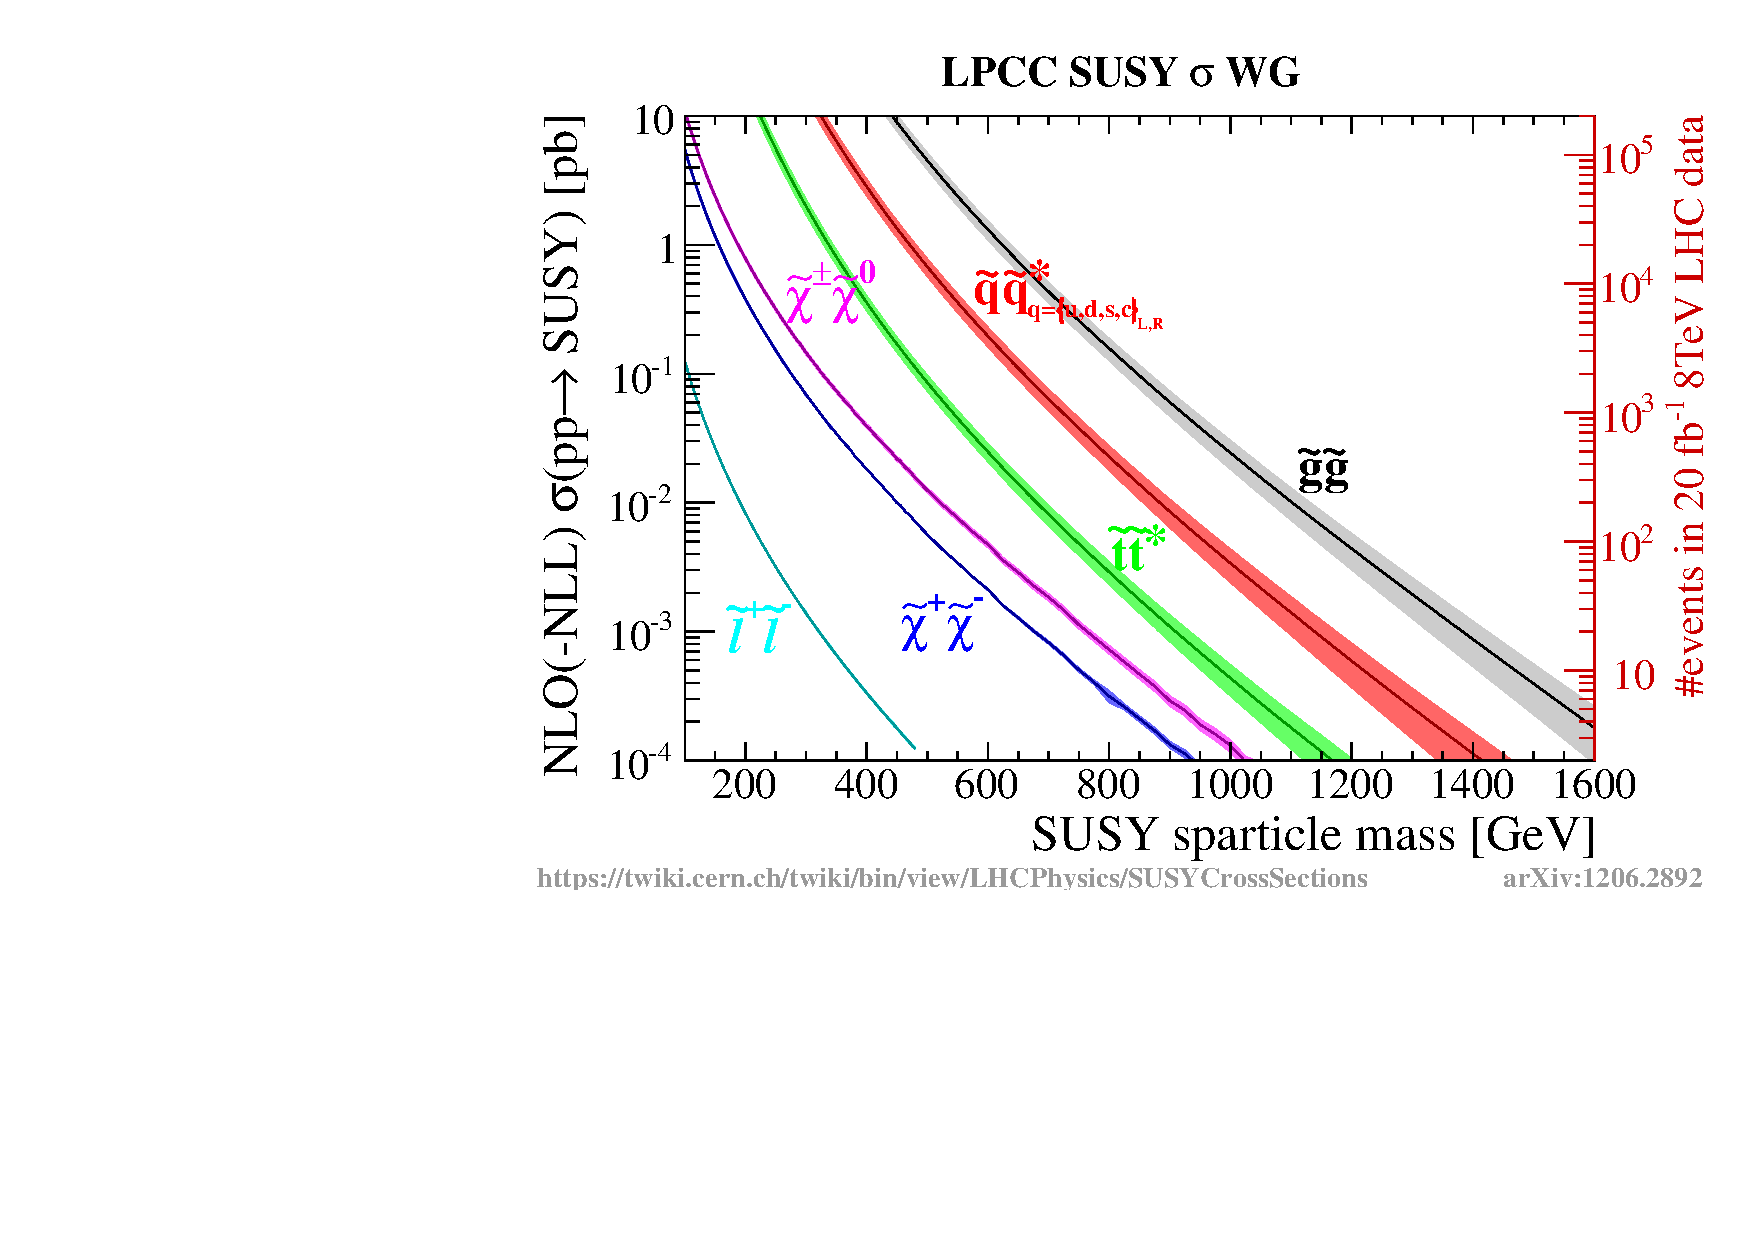
\includegraphics[width=0.8\textwidth]{figures/susy/xsections_strong}
  \caption{Cross sections for the production of various supersymmetric particles at a
centre-of-mass energy of 8\TeV. The expected number of produced events for a dataset of 20\fbinv
are also shown. Figure taken from~\cite{Kramer:2012bx}.
  \label{fig:susy_cross_sections}}
\end{figure}

At the LHC, the production of squarks and gluinos is dominated the gluon-gluon and gluon-quark
fusion. Once produced, they decay as explained in the previous section, possibly resulting in a
long decay cascade in which quarks and leptons can be produced. The full decay chain ends with
the production of at least two LSP's due to the conservation of R-parity. 
When this LSP is a neutralino, it will escape from the detector without being detected. This
will result in an imbalance of transverse momentum, which is one of the most powerful
discriminating variables in the search for SUSY signals. 

In general, SUSY signatures can contain any number of jets, leptons, and gauge bosons, depending on
the details of the mass spectrum. The SUSY search program at the CMS and ATLAS experiments therefore
covers a wide variety of final state topologies. Each analysis will be more or less sensitive to
certain classes of SUSY parameter points, and it is thus of extreme importance to search everywhere,
in all possible ways. The results of these searches can then be interpreted as limits on the
allowed SUSY parameter space. 





\section{Natural SUSY \label{sec:susy_natural_susy}}


Let us now come back to the hierarchy problem. As we have discussed before, radiative corrections
to the Higgs boson mass have the tendency to drive this mass up to very high scales in the SM. When
 supersymmetry is added to the theory, the quadratic contributions disappear due to the symmetries
with the fermions and bosons that run in the loop. However, there are still logarithmic dependencies
on the cutoff scale when SUSY is broken and the masses of the superpartners differ. 
The main contribution to the Higgs mass correction comes from the top quark and top squark loops,
due to the large Yukawa coupling. One can show that the top squark contribution has the general
form,
\begin{equation}
  \Delta m_{H_u}^2 \propto - \frac{3}{8\pi^2} y^2_t \left( m^2_{Q_3} + m^2_{\cPqu_3} + |A_t|^2 
  \right) \log \frac{\Lambda}{1\TeV} .
\end{equation}
Requiring that this term does not become too large, results in a bound on the stop mass of roughly
one \TeV. A similar reasoning can be made for the gluino, which contributes at one-loop level to the
top squark correction, and thus at two-loop level to the Higgs mass correction. The bound for
gluinos to be still considered natural is around 1.5\TeV. 
The $\mu$ parameter also has a big effect on the Higgs boson mass corrections, as it contributes
already at tree-level. The bound on $\mu$, and thus the higgsinos, is of the order of 300\GeV. 

With these considerations in mind, \textit{natural SUSY}~\cite{Barbieri:2009ev,Papucci:2011wy} can
be defined as the subset of the SUSY parameter space for which the above constraints on the
sparticle masses are fulfilled. 
A natural SUSY scenario has low finetuning, and thus resolves the hierarchy problem. A typical mass
spectrum is shown in Fig.~\ref{fig:natural_spectrum}. The idea of natural SUSY has driven many
searches at the LHC, and has drawn particular attention to searches for gluinos and third
generation squarks, as those particles are the only strongly produced particles that are required
to be relatively light. 


\begin{figure}[t]
  \centering
  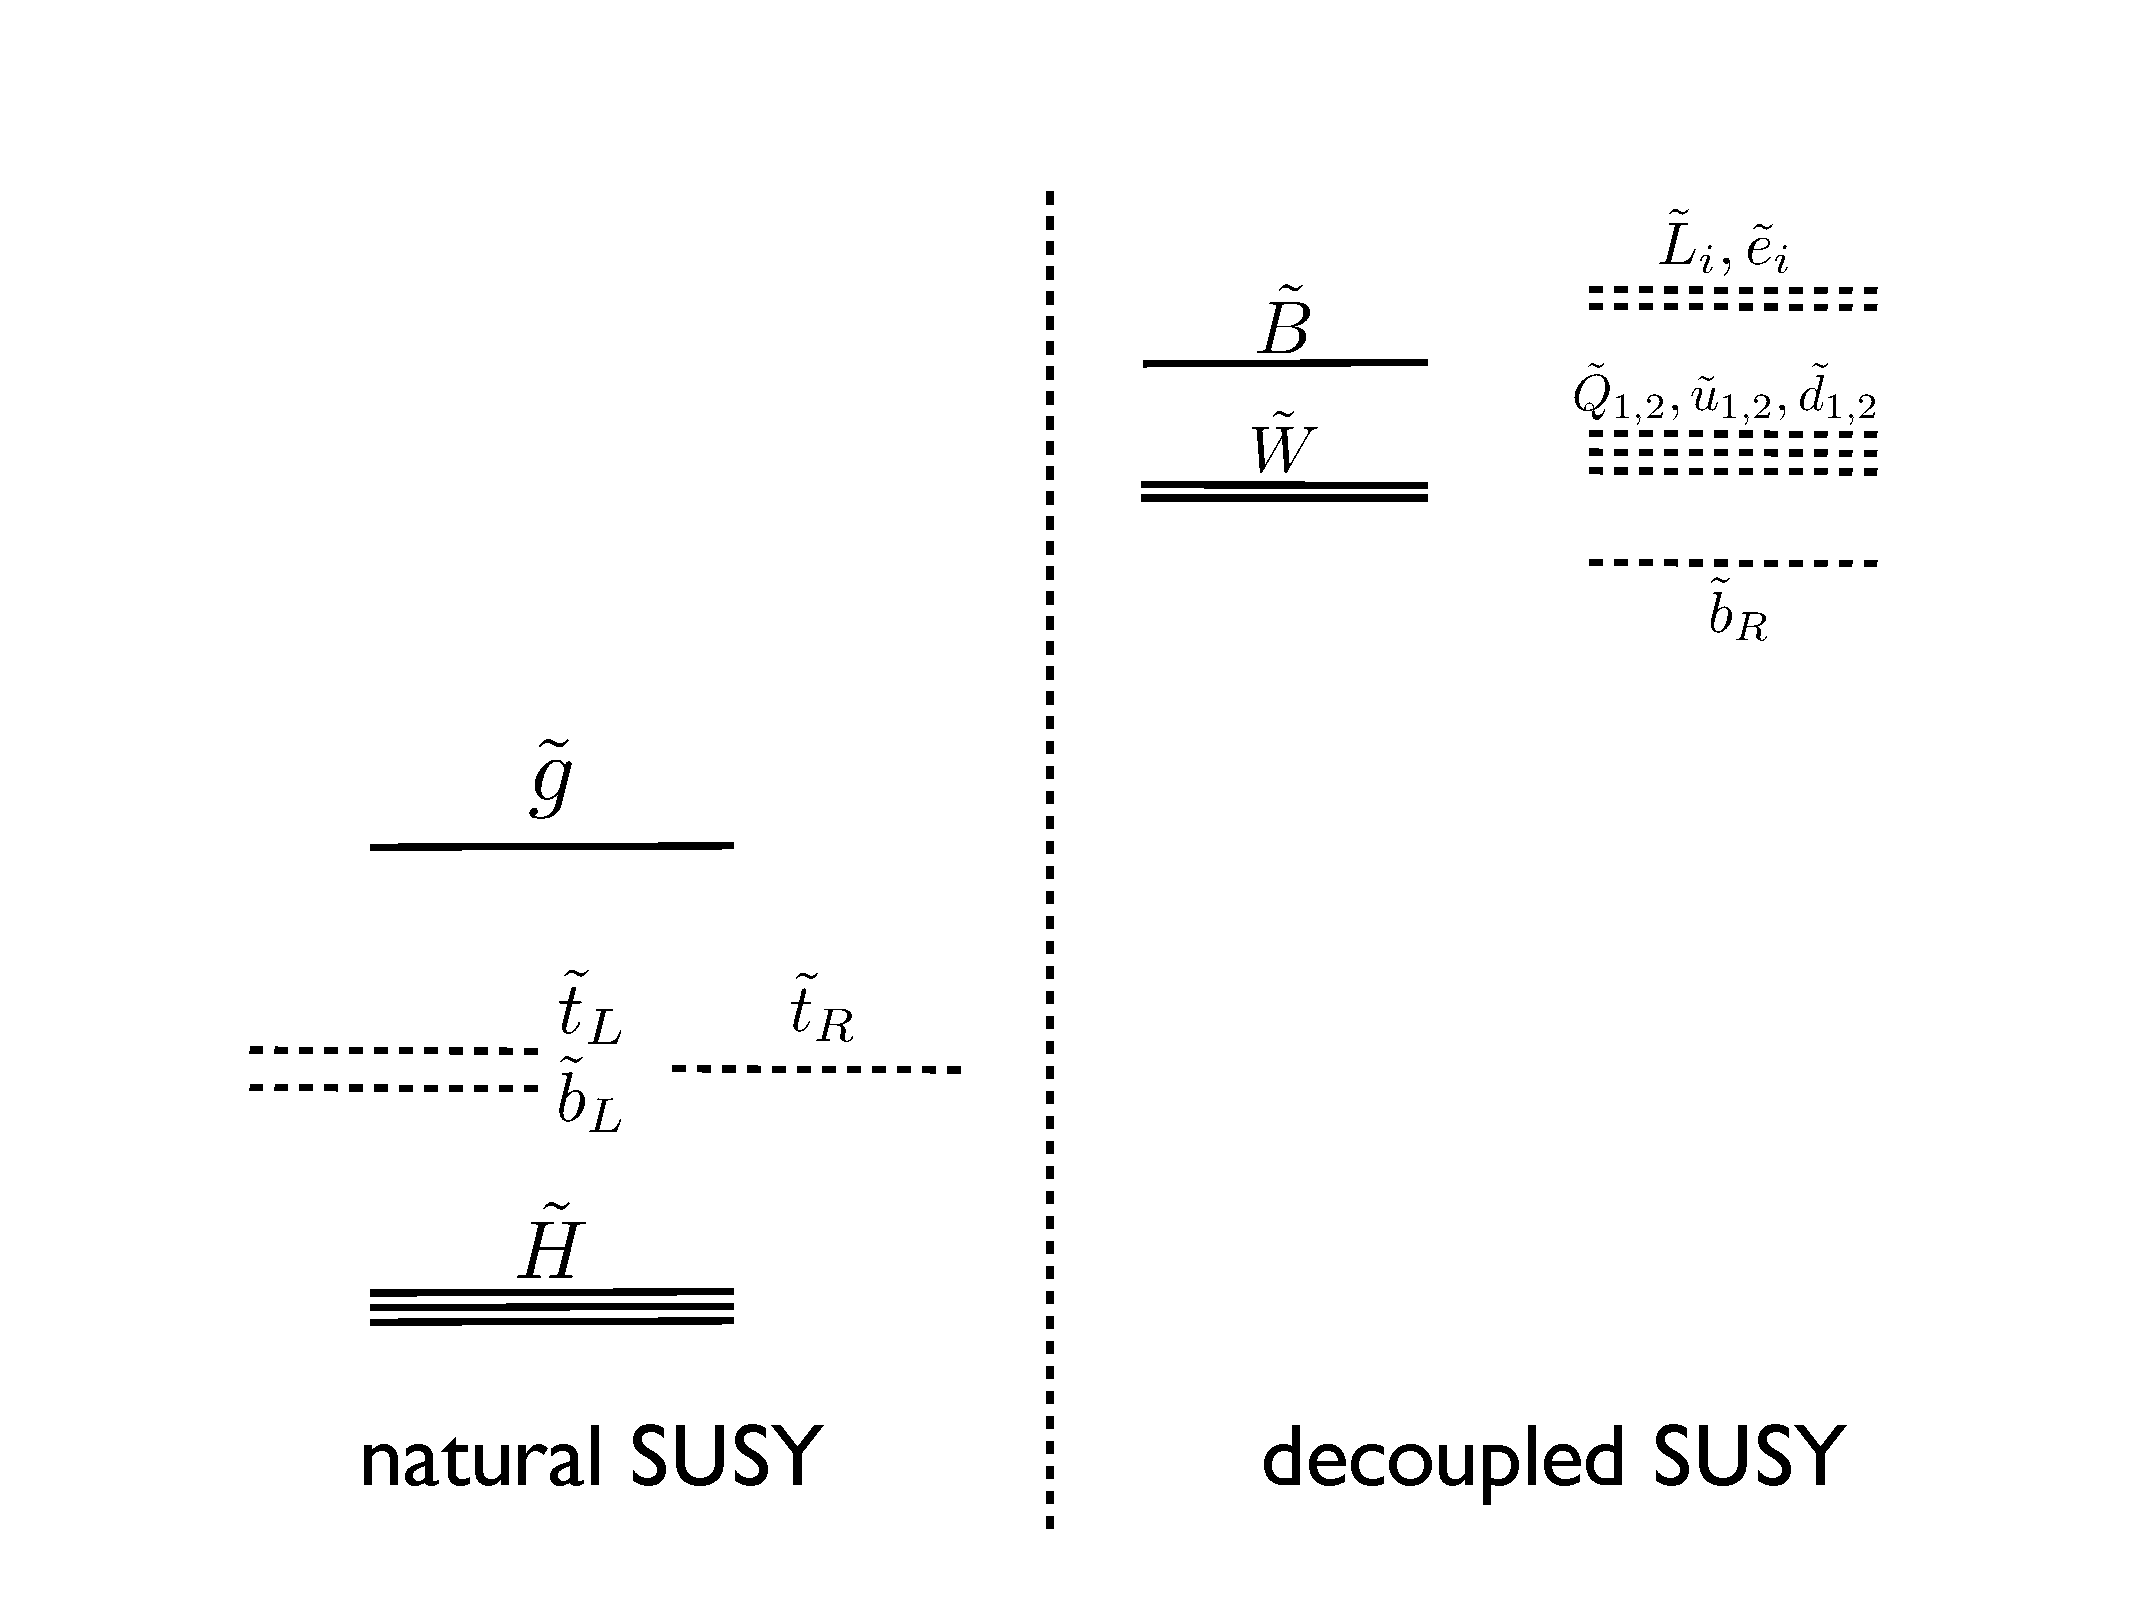
\includegraphics[width=0.8\textwidth]{figures/susy/NaturalSpec}
  \caption{ A natural SUSY spectrum, containing light higgsinos, light top squarks, and a light
gluino. All other superpartners can be decoupled at high masses. Figure taken from
Ref.~\cite{Papucci:2011wy}.
  \label{fig:natural_spectrum}}
\end{figure}


%%%%%%%%%%%%%%%%%%%%%%%%%%%%%%%%%%%%%%%%%%%%%%%%%%%%%%%%%%%%%%%%%%%%%%%%%%%%%%%%%%%%%%%%%%%%%%%%%%%

\section{Simplified model spectra \label{sec:susy_sms}}

Many extensions of the Standard Model are possible, and many of the models have numerous free
parameters. The MSSM is no exception. Without additional simplifications there are 104 extra free
parameters; with a minimal set of assumptions, there are still about 20 parameters left. This
extremely large parameter space is not very practical to do an analysis. 
Furthermore, similar experimental signatures can be produced in different ways, and by different
models.
To address these issues, a simplified approach was developed, using the so-called
\textit{simplified model spectra} (SMS)~\cite{Alves:2011wf,Alwall:2008ag,Chatrchyan:2013sza},
rather than full models. These SMS are based primarily on the experimental topologies, how many jets
or leptons are produced, whether there are jets originating from $\cPqb$ quarks, etcetera. 

Simplified models only contain a limited number of particles and interactions, and can be modelled
as an effective theory. 
The result is a very minimal set of parameters for which no assumptions on relations between
parameters have been made. This makes the simplified models both simpler, and more general.
They are more suitable to optimize and interpret a new physics search compared to a full-fledged
new physics model, for which, depending on assumptions, key topologies could be missing.
The purpose of simplified models is three-fold,
\begin{itemize}
  \item Identifying the boundaries of the search sensitivity. By scanning different masses, or mass
differences between particles, it becomes easier to identify where searches lose sensitivity. This
can then be used as input in the proposal of new dedicated analyses. 

  \item Characterizing possible new physics signals. If a signal is observed, SMS's can be used as
a starting point to quantify the compatibility with different kinds of processes. Starting the
characterization with full models would be very cumbersome due to the many free
parameters that would need to be scanned.

\item Derive limits on more general models. Complex models can be decomposed into experimental
final state topologies. Ideally, each of those topologies would correspond to a SMS. The exclusion
limits on the simplified models can then be translated back into a limit on the full model. 
Several efforts in this respect exist within the phenomenology community, such as
SModelS~\cite{Kraml:2013mwa,Kraml:2014sna}, Fastlim/ATOM~\cite{Papucci:2014rja}, and
checkMATE~\cite{Kim:2015wza}.
\end{itemize}


Let us consider as example a simplified model that only includes a gluino and the lightest
neutralino. We further assume that the gluino can only decay as $\tilde{g}\rightarrow \cPq \cPaq
\lsp$. Simplified models are described by effective theories, in this example the decay
proceeds through the dimension-six operator, 
\begin{equation}
  \mathcal{L}_{\text{int}} = \frac{\lambda_i^2}{M_i^2} \tilde{g} \cPq_i \cPaq_i \lsp + h.c. , 
\end{equation}
where $i$ runs over the different quark flavours, $\lambda_i$ is the Yukawa coupling for the
quark-squark-$\lsp$ vertex, and $M_i$ is the effective scale of the interaction. 
Collision events can be simulated according to this effective Lagrangian in two main ways. The
first is through the use of programs such as \textsc{marmoset}~\cite{ArkaniHamed:2007fw}, which
allows to directly simulate the on-shell effective theory. 
The second, and most widely used, way is to use a matrix element generator, such as \MADGRAPH (see
Section~\ref{sec:event_matrix_element_generators}), to simulate events using the MSSM as model,
setting the masses for all particles that are not involved in the SMS to very high values of
$\mathcal{O}(100\TeV)$.
Any diagrams involving particles not included in the SMS will then effectively not contribute at
all, and the MSSM will be reduced to the SMS under study.  
No matter the details of the simulation, the only parameters that are relevant for this SMS are the
gluino production cross
section, the branching ratio for the decay (here assumed to be 100\%), and the masses for the gluino
and the $\lsp$. Analyses will then usually make a two-dimensional scan across the
($\tilde{g},\lsp$) mass plane, and investigate how their sensitivity changes.


We also note that although the simplified models are SUSY-inspired, and use the SUSY nomenclature,
they are in fact more general. Any model containing a spectrum of new narrow resonances, with the
same gauge and flavour quantum numbers as the SM, and that are odd under some conserved parity, fits
within the scope of the simplified models. Non-SUSY examples are the little Higgs models with
T-parity, or universal extra dimensions with KK-parity. 



 